\begin{frame}[fragile]{Arrows (1)}
\centering Another way to think about computations:
\begin{center}
	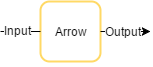
\includegraphics[scale=0.8]{images/arrow}~\\
\end{center}
\end{frame}

\begin{frame}[fragile]{Arrows (2)}
\begin{minipage}{0.6\textwidth}
\begin{lstlisting}[frame=htrbl, numbers=none]
class Arrow arr where
	arr :: (a -> b) -> arr a b
	
	
	
	(>>>) :: arr a b -> arr b c -> arr a c
	
	
	
	
	first :: arr a b -> arr (a,c) (b,c)
\end{lstlisting}
\vfill
\end{minipage}
\hspace*{0.03\textwidth}
\begin{minipage}{0.25\textwidth}
	~\\~\\~\\
	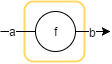
\includegraphics[scale=0.6]{images/arr}~\\~\\
	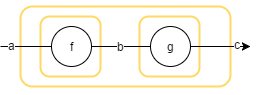
\includegraphics[scale=0.6]{images/compose}~\\~\\
	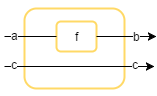
\includegraphics[scale=0.6]{images/first}~\\~\\
\end{minipage}
\end{frame}

\begin{frame}[fragile]{Arrow Example}
	Arrow usage example:
\begin{lstlisting}[frame=htrbl]
add :: Arrow arr => arr a Int -> arr a Int -> arr a Int
add f g = (f &&& g) >>> arr (\(u, v) -> u + v)
\end{lstlisting}
	\begin{center}
		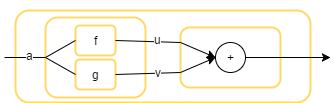
\includegraphics[scale=0.6]{images/addA-comb}
	\end{center}
\end{frame}